\documentclass{article}


\usepackage[french]{babel}
\usepackage[utf8]{inputenc}

\usepackage[a4paper,top=2cm,bottom=2cm,left=3cm,right=3cm,marginparwidth=1.75cm]{geometry}


\usepackage{amsmath}
\usepackage{graphicx}
\usepackage[colorlinks=true, allcolors=blue]{hyperref}
	
\usepackage{listings}

\title{Première version du cahier d’analyse des besoins à propos d'un programme de jeux d'échecs}
\author{Rossignon Morgan, Daniel Karl, Salomode Florian, Beites Marvin, Zucchelli Thomas}

\begin{document}

\maketitle
\centerline{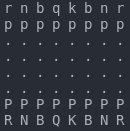
\includegraphics[scale = 1]{echecs_title.png}}

\tableofcontents
\newpage

\section{Objectifs généraux du projet}
Le but du projet est de programmer un joueur d'échec complet en appliquant les algorithmes les plus fréquents et en utilisant au mieux les bitboards. L'interface utilisateur sera purement en mode texte (ce n'est pas le but du projet). Si possible, plusieurs approches pourront être implantées et comparées via des tournois entre les différentes stratégies.

Le projet se dirigera vers des techniques d'exploration d'arbre classiques telles que Minimax-
ab, Negamax, Negascout, MTD(f), Monte-Carlo Tree Search (MCTS). Ainsi qu'au développement d'heuristiques propres au jeu.

\subsection{Pseudo-code des différentes techniques d'exploration d'arbre classiques : }
\medskip
\subsubsection{Minimax-ab :}
\centerline{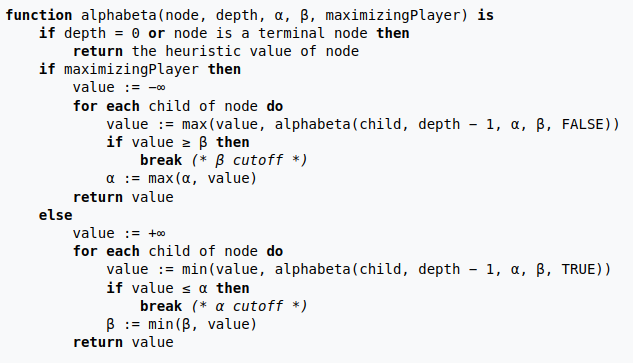
\includegraphics[scale = 0.5]{Alpha_beta_minmax.png}}
\medskip
\subsubsection{Negamax : }
\centerline{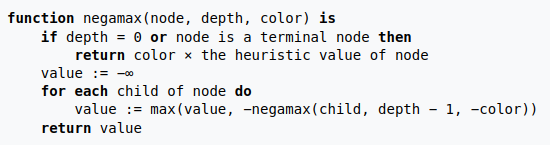
\includegraphics[scale = 0.5]{Negamax_1.png}}
\centerline{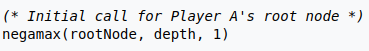
\includegraphics[scale = 0.5]{Negamax_2.png}}
\centerline{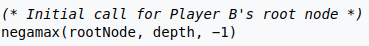
\includegraphics[scale = 0.5]{Negamax_3.png}}
\medskip
\subsubsection{Negascout : }

\centerline{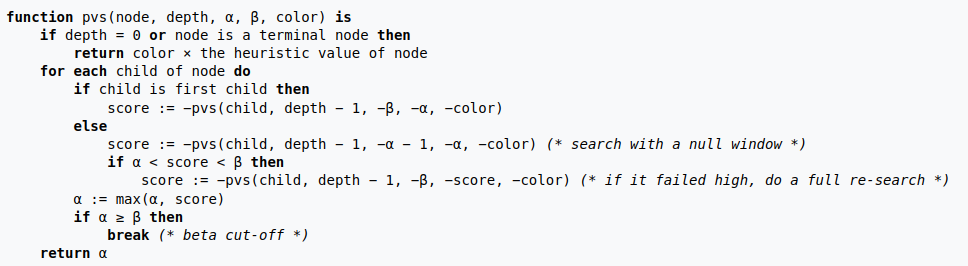
\includegraphics[scale = 0.5]{Negascout.png}}
\medskip
\subsubsection{MTD(f) : }

\centerline{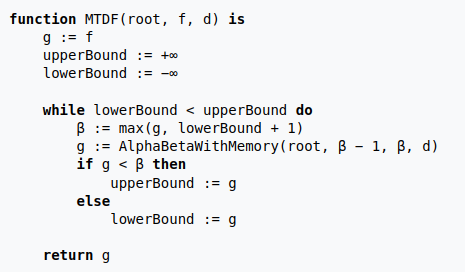
\includegraphics[scale = 0.5]{MTDf.png}}
\medskip
\subsubsection{Monte-Carlo Tree Search (MCTS) : }

\centerline{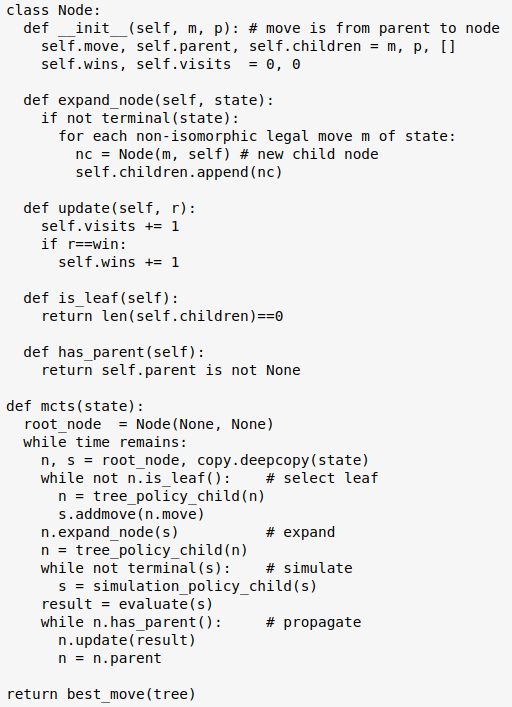
\includegraphics[scale = 0.5]{Monte_carlo_tree_search.png}}

\newpage
\section{Analyse de l'existant}
\centerline{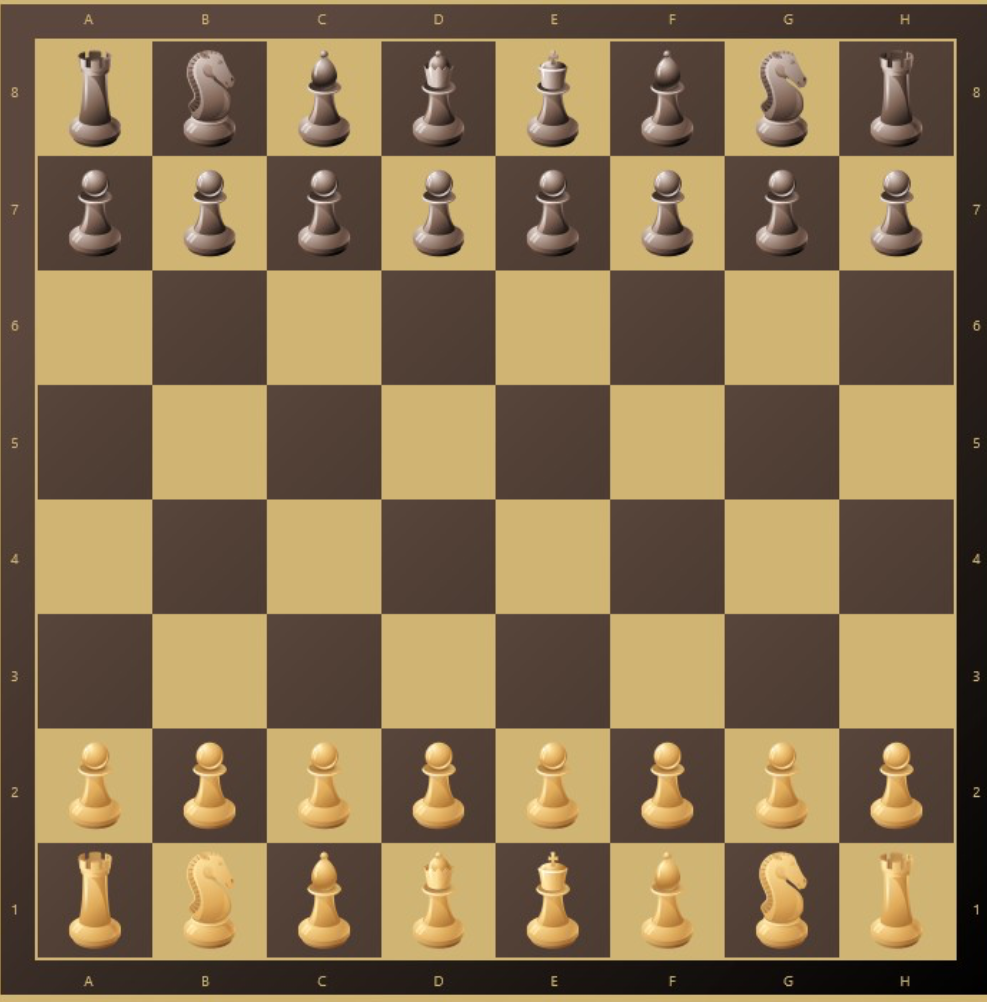
\includegraphics[scale = 0.25]{Echiquier.png}}
La plupart des logiciels de jeu d'échec optent pour un affichage graphique afin de jouer aux échecs, toutefois on peut se rendre compte que ces logiciels permettent aux joueurs de :
\begin{itemize}
\item sélectionner qui joue en premier. (qui joue les pièces blanches)
\item sélectionner le nombre de joueurs. (l'ia contre l'ia, 1 joueur contre l'ia ou 2 joueurs)
\item sélectionner une difficulté pour l'ia.
\newline{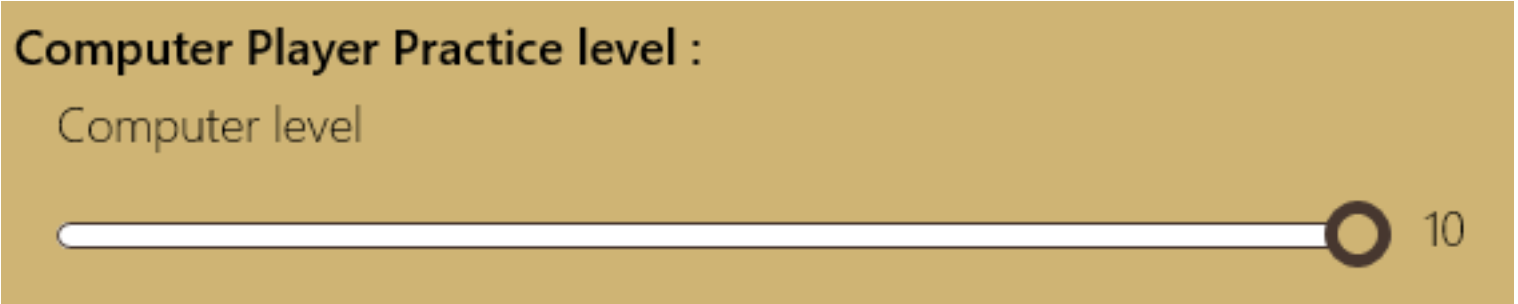
\includegraphics[scale = 0.5]{Computer_level.png}}
\item visualiser les mouvements d'une pièce
\newline
\centerline{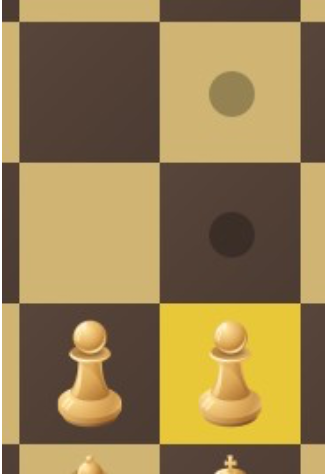
\includegraphics[scale = 0.5]{Piece_move.png}}
\item sauvegarder une partie pour la reprendre plus tard. -charger une partie sauvegardée.
\end{itemize}


\newpage
\section{Description des besoins}

%Éventuellement avec distinction besoins
%utilisateurs/besoins système.

%Ces besoins seront expliqués, justifiés, illustrés au moyen de : scénarios,
%prototypes (par ex. prototypes papier pour les interfaces, prototypes
%implémentés pour la faisabilité)
\begin{itemize}

\subsection{Liste des besoins fonctionnels}
\medskip
%chacun associés à :
%- Un niveau de priorité d’implémentation dans le projet.
%- Toutes ou une partie des rubriques (a)-(e) ci-dessous.

%Analyse de source (lecture de fichier ?...), récupération des graphes de dépendances (ou création suite à l'analyse de source ?...),  affichage des graphes.
    \item \textbf{Création du plateau de jeu : }
    \medskip
    \begin{itemize}
        \item Représentation du plateau à l'aide de bitboards \cite{Bitboards}, chaque bitboard représentera l'emplacement des pièces d'un même type et d'une même couleur. ( c-a-d qu'il y aura un bitboard pour l'emplacement de tous les pions blanc, un bitboard pour l'emplacement de tous les Cavaliers blanc,...).
    \end{itemize}
    \medskip
    \item \textbf{Afficher le plateau de jeu : }
    \medskip
    \begin{itemize}
        \item Affichage en texte, une lettre représente un pion (p = pion, k = roi, q = reine,
b = fou, r = tour, n = cavalier).
        \item Afin de différencier les pions des 2 joueurs du plateau de jeu, le joueur 1 aura des pions en majuscule et le joueur 2 en minuscule.
        \item Les coordonnées des cases sont visibles sur les côtés de la grille, les numéros représentent les lignes et les lettres majuscules pour les colonnes, par exemple (1A = 1ère case en haut à gauche \dots).
    \end{itemize}
    \medskip
    \item \textbf{Lister les mouvements possibles : }
    \newline
        Une commande permet d'afficher la liste de tous les coups jouables pour l'utilisateur ( par exemple : 2A3A \dots).
    \medskip
    \item \textbf{Déplacer une pièce : }
    \newline
    Le programme doit faire respecter les règles du jeu aux différents algorithmes, ou joueur humain.
    Le déplacement d'une pièce doit vérifier au préalable que le mouvement est possible, et si c'est le cas, ce que ce mouvement engendre.
    \begin{enumerate}
        \item Le programme doit vérifier que le mouvement demandé correspond à un des mouvements possibles de la pièce.
        \item Si le mouvement est correct pour la pièce, il doit vérifier que la case n'est pas occupé par une pièce alliée (de la même couleur), auquel cas, le mouvement n'est pas valide.
        \item Si la case n'est pas occupée par une pièce alliée, le programme vérifie si une pièce ennemie 
        se trouve sur la case. 
        Si c'est le cas la pièce ennemie est détruite du plateau de jeu.
        \item Enfin, la pièce se déplace sur la case cible.
    \end{enumerate}
    \medskip
    \item \textbf{Garder une trace de l'historique : }
    \newline
        Le programme doit garder en mémoire les 6 derniers plateaux de jeux (3 derniers coups de chaque joueurs) afin de les comparer et d'annoncer un match nul si le même plateau est répété 3 fois. 
    \medskip
    \item \textbf{Choisir les algorithmes à utiliser : }
        \newline
        En début de partie, une liste des différents algorithmes est proposée à l'utilisateur qui n'a plus qu'à recopier dans le terminal celle contre qui il veut jouer ou tout simplement celles qu'il veut voir s'affronter, ainsi que ses paramètres ( profondeur de recherche, attribution des rôles Joueur\_1 et Joueur\_2 \dots).
    \medskip
    \item \textbf{Afficher des statistiques :
    }
        \newline
        Le logiciel doit pouvoir afficher les statistiques de la dernière partie lancée. 
        \newline
        Il faudra donc que le logiciel affiche le type d'algorithme utilisé et ses paramètres, quelle ia a gagné ou non, le nombre de tours pour finir la partie, pour chaque tour le temps pris par les ia ou joueurs pour réaliser une action, et le temps moyen d'un tour des ia.
    \medskip
    \item \textbf{Lancer un tournois entre algorithmes : }
    \newline
        Il est possible de lancer un tournois entre différents algorithmes afin de voir lequel est le plus performant.
        \newline
        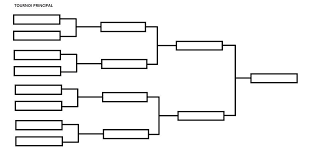
\includegraphics[scale = 1]{tournoi.png}
        \newline
        À la suite de ce tournoi, une liste de commandes est proposée à l'utilisateur afin de consulter les 
        statistiques des matchs de chaque algorithme (nombre de coups avant la victoire \dots).
    \medskip
    \item \textbf{Lancer des Algorithmes sur des énigmes : }
    \newline
        Dans le monde des Échecs il existe des "problèmes" d'échec \cite{Krt}, c-à-d d'après un plateau donné il faut réussir à mettre en place des stratégies comme mettre le roi adverse en échec en un certain nombre de coups.\newline
        il sera donc possible de lancer les algorithmes sur ces "problèmes". 
\end{itemize}



\subsection{Liste des besoins non-fonctionnels}
\medskip
\begin{itemize}
    
    \item \textbf{Performances : }
    Une partie jouée entre deux Algorithmes ne doit pas non plus durer des heures, les algorithmes ne devrons pas dépasser un certain temps pour chaque coup.
    \newline
    \item \textbf{Fiabilité : }
    Éviter que le jeu crash \dots
    \newline
    \item \textbf{Facilité d'utilisation : } 
    Toutes les commandes possibles doivent être listées à l'utilisateur, ainsi que leurs fonctions, afin de le guider et qu'il ne perde pas de temps à comprendre le fonctionnement du programme.
    \newline
    \item \textbf{Domaine d'action : } 
    Les utilisateurs sont lambda (pas forcément des informaticiens) mais il faut quand même qu'ils sachent utiliser un terminal car nous n'avons pas d'interface graphique.
    \newline
    \item \textbf{Portabilité : } 
    \newline
    Le programme doit être exécutable sous tout système d'exploitation permettant de coder ou exécuter du C. 
    \newline
    \item \textbf{Contraintes d'interopérabilité : } 
    \newline
    \item \textbf{Contraintes légales : } 
\end{itemize}


\bibliographystyle{unsrt}
\bibliography{sample}

\end{document}